\section{Results and Findings}
\label{sec:eval}

This section describes our experiment results and findings.  We (1)
describe the training details of our experiment, including the
environment and hyper-parameters, (2) show the results for \comgen and
\methnam tasks, and (3) list the key observations and findings from
our experiment.

\subsection{Training Details}
\label{sec:eval:hyparam}

We trained and tested all models on a super computer, where each model
use a NVIDIA GTX 1080-TI GPU and four models share two Intel(R)
Xeon(R) CPU E5-2620 CPUs and 128GB of RAM.  We trained and tested each
model in each evaluation setting \NumTrial times and each run is
initialized using different random seed.

We followed the source literature to setup the hyper-parameters of
models. \Fix{...}

\subsection{Results for \ComGen}
\label{sec:eval:results-comgen}


%% Automatically generated by pyutil.latex 

\begin{table*}
\begin{small}
\begin{center}
\caption{\TCResultsComGen}
\begin{tabular}{l|rr|rr|rr}
\toprule
 & \multicolumn{2}{c|}{\UseMacro{TH-exp-mixedproj-2020}}
 & \multicolumn{2}{c|}{\UseMacro{TH-exp-crossproj-2020}}
 & \multicolumn{2}{c}{\UseMacro{TH-exp-evo-2020}}
\\
\multirow{-2}{*}{\THModel} 
 & \UseMacro{TH-metric-bleu}
 & \UseMacro{TH-metric-xmatch}
 & \UseMacro{TH-metric-bleu}
 & \UseMacro{TH-metric-xmatch}
 & \UseMacro{TH-metric-bleu}
 & \UseMacro{TH-metric-xmatch}
\\
\midrule
\UseMacro{TH-model-Seq2seq}
 & \UseMacro{mixedproj-2020-test_common-bleu-Seq2seq-AVG}
 & \UseMacro{mixedproj-2020-test_common-xmatch-Seq2seq-AVG}$^{\gamma\epsilon}$
 & \UseMacro{crossproj-2020-test_common-bleu-Seq2seq-AVG}
 & \UseMacro{crossproj-2020-test_common-xmatch-Seq2seq-AVG}
 & \UseMacro{evo-2020-test_common-bleu-Seq2seq-AVG}
 & \UseMacro{evo-2020-test_common-xmatch-Seq2seq-AVG}$^{\zeta\theta}$
\\
\UseMacro{TH-model-Seq2seqAtt}
 & \UseMacro{mixedproj-2020-test_common-bleu-Seq2seqAtt-AVG}$^{\alpha}$
 & \UseMacro{mixedproj-2020-test_common-xmatch-Seq2seqAtt-AVG}$^{\delta\epsilon}$
 & \UseMacro{crossproj-2020-test_common-bleu-Seq2seqAtt-AVG}
 & \UseMacro{crossproj-2020-test_common-xmatch-Seq2seqAtt-AVG}
 & \UseMacro{evo-2020-test_common-bleu-Seq2seqAtt-AVG}$^{\beta}$
 & \UseMacro{evo-2020-test_common-xmatch-Seq2seqAtt-AVG}$^{\eta\theta}$
\\
\UseMacro{TH-model-DeepCom}
 & \UseMacro{mixedproj-2020-test_common-bleu-DeepCom-AVG}$^{\alpha}$
 & \UseMacro{mixedproj-2020-test_common-xmatch-DeepCom-AVG}$^{\gamma\delta}$
 & \UseMacro{crossproj-2020-test_common-bleu-DeepCom-AVG}
 & \UseMacro{crossproj-2020-test_common-xmatch-DeepCom-AVG}
 & \UseMacro{evo-2020-test_common-bleu-DeepCom-AVG}$^{\beta}$
 & \UseMacro{evo-2020-test_common-xmatch-DeepCom-AVG}$^{\zeta\eta}$
\\
\bottomrule
\end{tabular}
\end{center}
\end{small}
\vspace{\TVResultsComGen}
\end{table*}


Table~\ref{table:results-com-gen} shows the automatic metrics (\bleu
and \xmatch) for each \methodology (\mixedproj, \crossproj, and
\evoaware) for the models we selected for the \comgen task.

\begin{figure}[t]
  \centering
  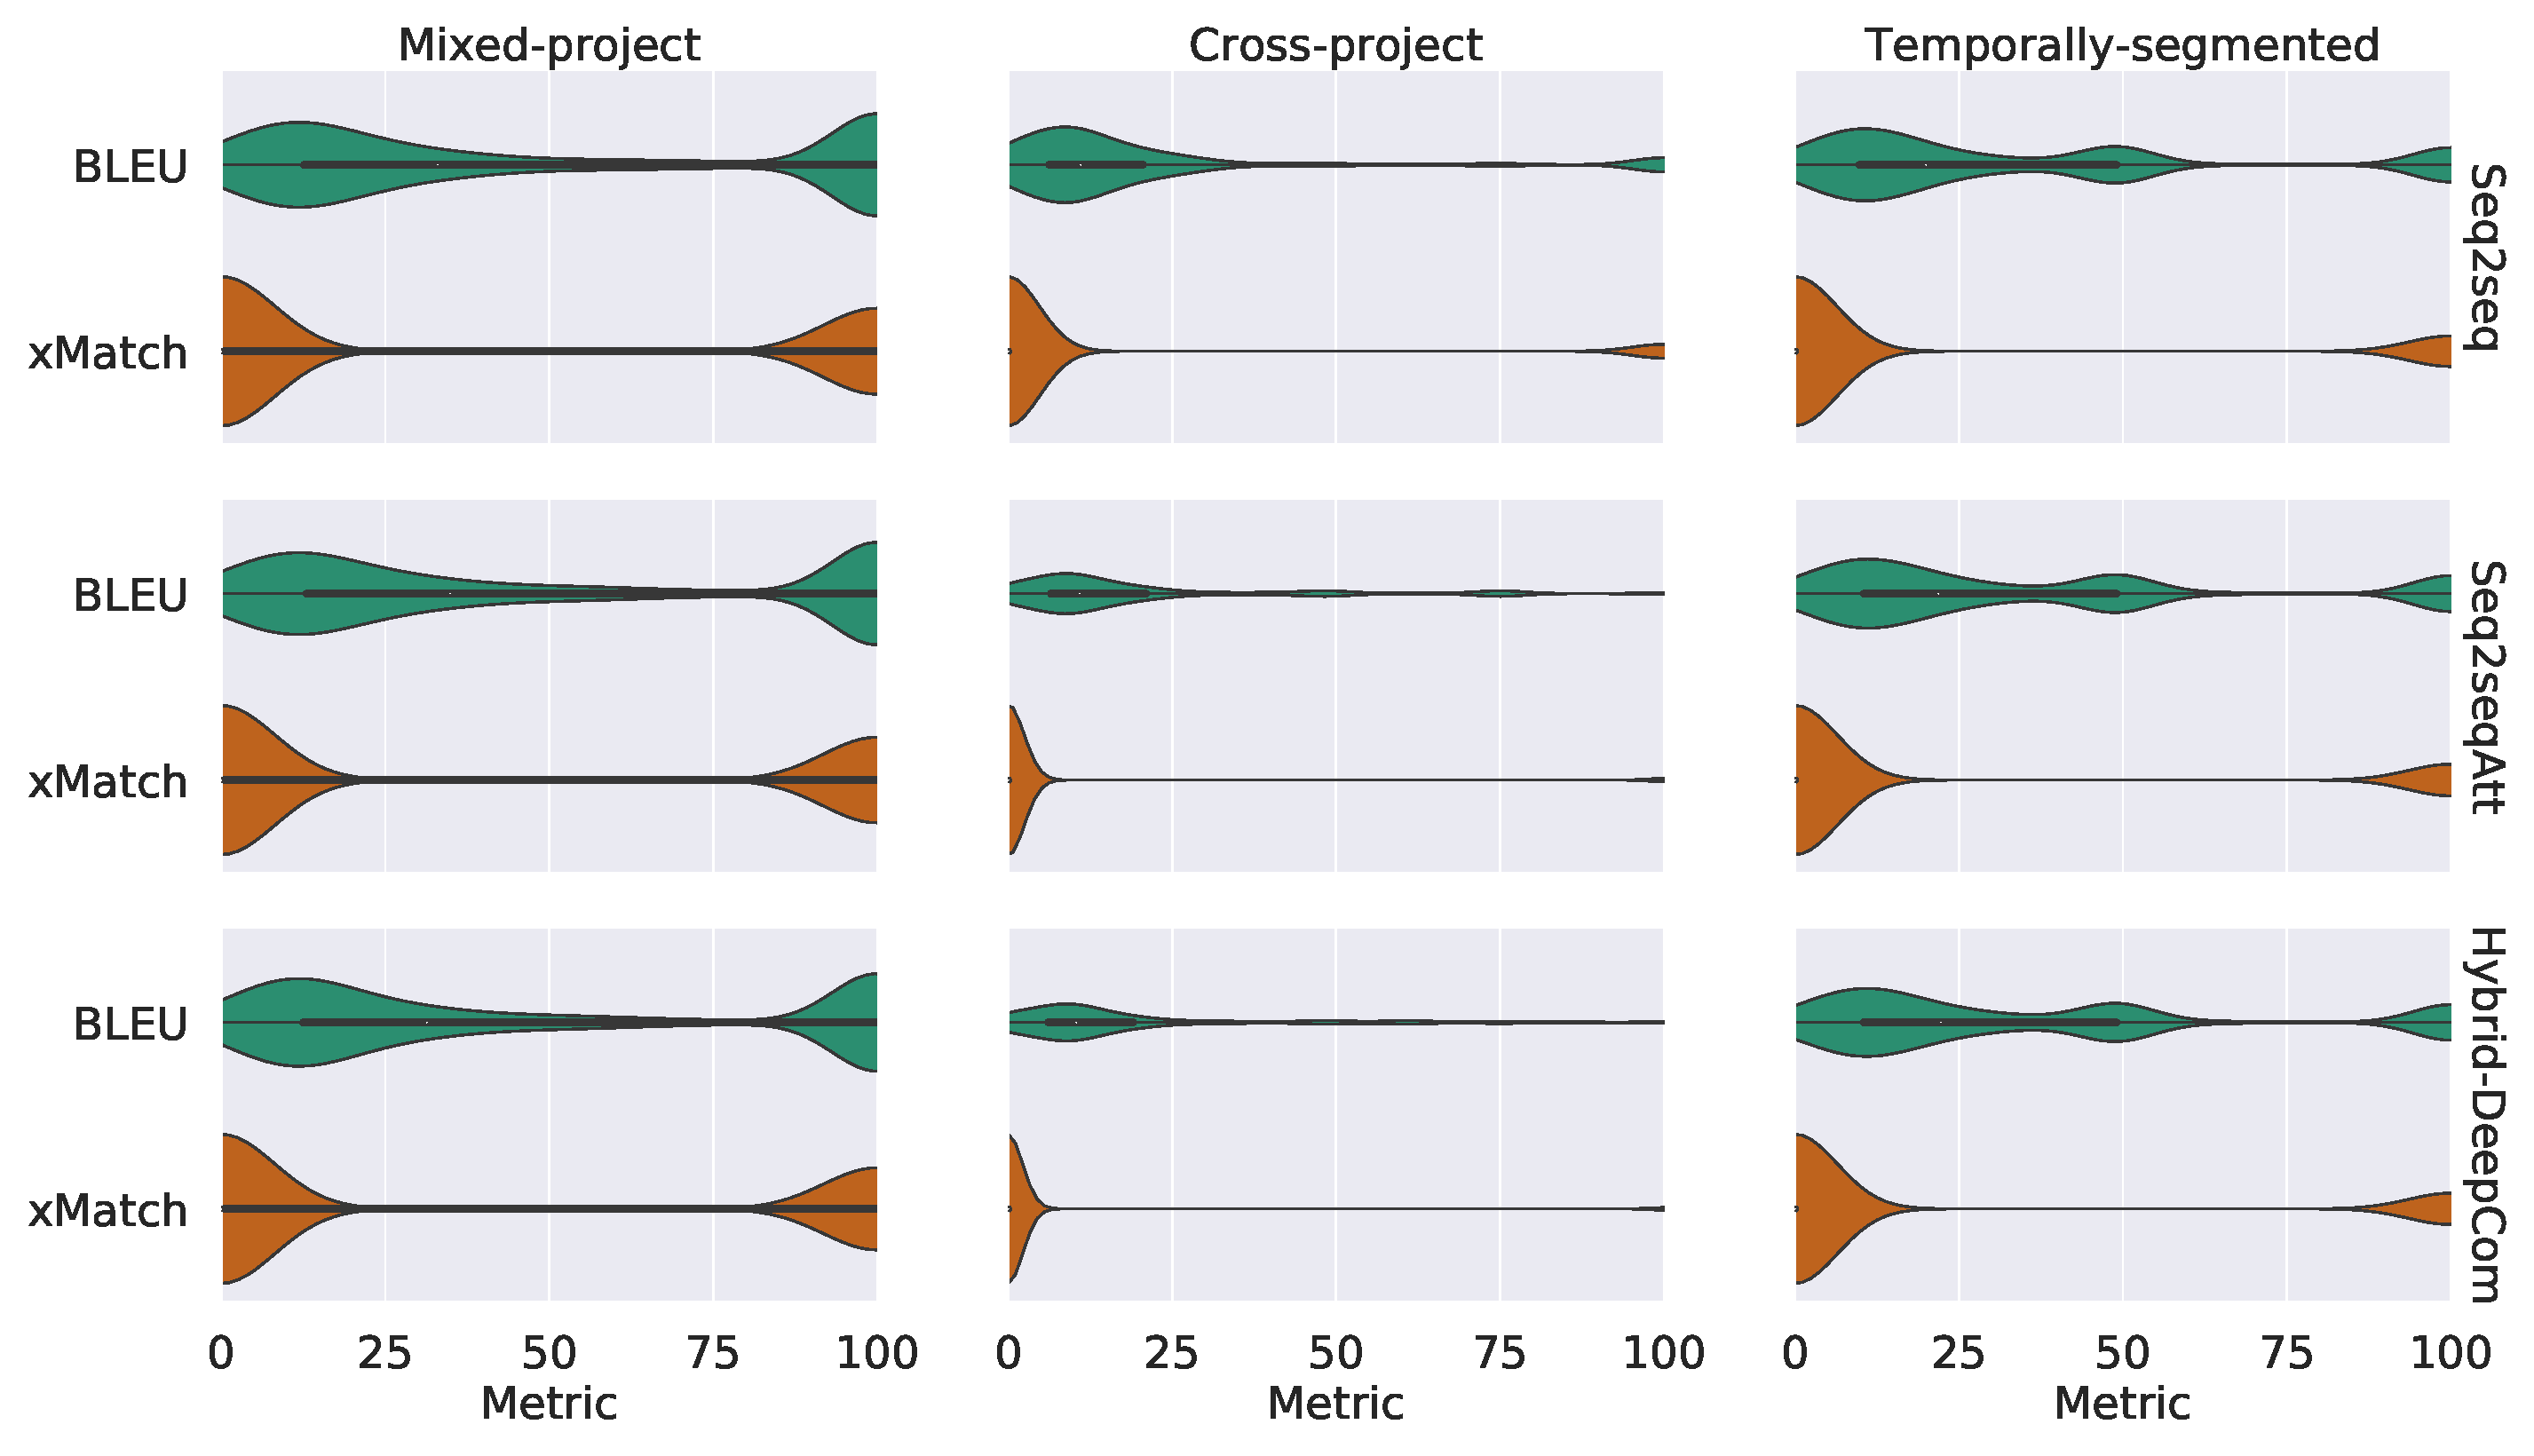
\includegraphics[width=\columnwidth]{figs/models-results-metrics-dist-ComGen.eps}
  \caption{Each violin plot shows the distribution of automated
    metrics on all examples in \test set.  Left to right: \mixedproj,
    \crossproj, and \evoaware \methodologies.  Top to bottom: the
    models for \comgen
    task. \label{fig:models-results-metrics-dist-ComGen}}
\end{figure}

\begin{figure}[t]
  \centering
  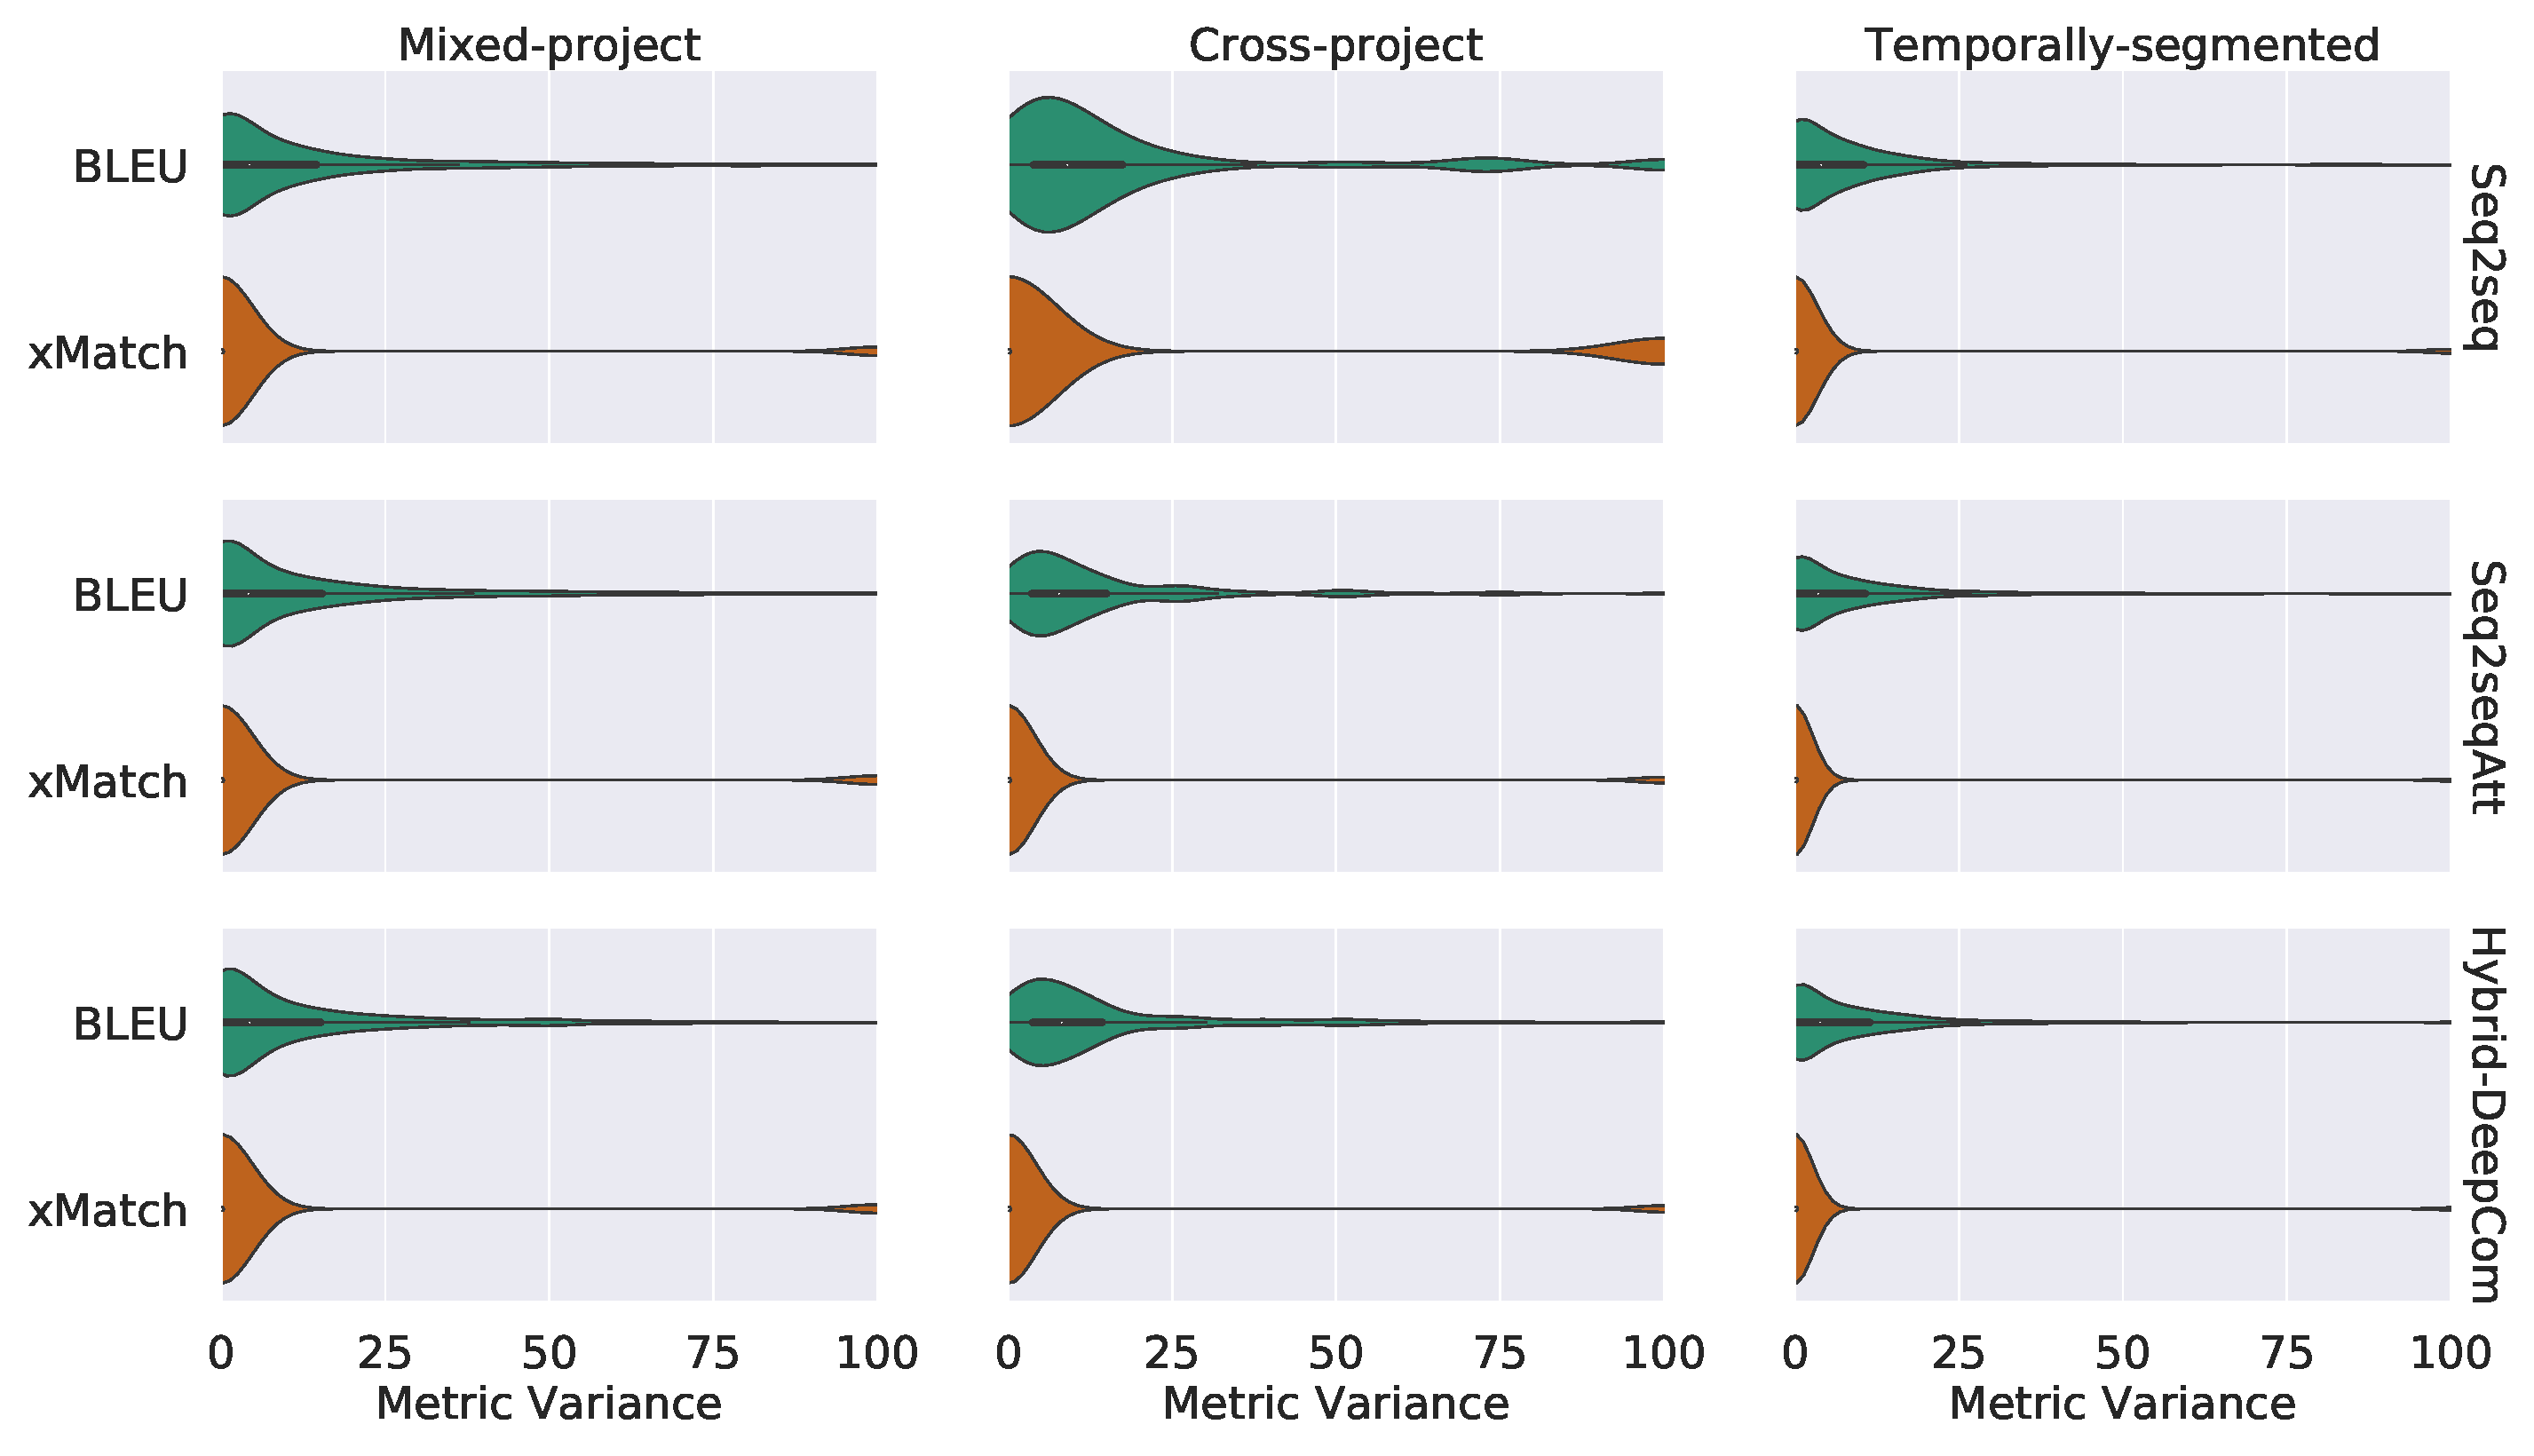
\includegraphics[width=\columnwidth]{figs/models-results-variance-dist-ComGen.eps}
  \caption{Each violin plot shows the distribution of the variances of
    automated metrics on all examples in \test set between \NumTrial
    trials.  Left to right: \mixedproj, \crossproj, and \evoaware
    \methodologies.  Top to bottom: the models for \comgen
    task. \label{fig:models-results-variance-dist-ComGen}}
\end{figure}

Figure~\ref{fig:models-results-metrics-dist-ComGen} shows the
distributions of automatic metrics on examples in \test set.
Figure~\ref{fig:models-results-variance-dist-ComGen} shows the
distributions of the variances of automated metrics on examples in
\test between \NumTrial different trials, where the variance is
calculated as the diff of the maximum value in \NumTrial trials and
minimum value in \NumTrial trials.


\subsection{Results for \MethNam}
\label{sec:eval:results-methnam}


%% Automatically generated by pyutil.latex 

\begin{table*}
\begin{small}
\begin{center}
\caption{\TCResultsMethNam}
\begin{tabular}{l|rrrr|rrrr|rrrr}
\toprule
 & \multicolumn{4}{c|}{\UseMacro{TH-exp-mixedproj-2020}}
 & \multicolumn{4}{c|}{\UseMacro{TH-exp-crossproj-2020}}
 & \multicolumn{4}{c}{\UseMacro{TH-exp-evo-2020}}
\\
\multirow{-2}{*}{\THModel} 
 & \UseMacro{TH-metric-f1}
 & \UseMacro{TH-metric-precision}
 & \UseMacro{TH-metric-recall}
 & \UseMacro{TH-metric-xmatch}
 & \UseMacro{TH-metric-f1}
 & \UseMacro{TH-metric-precision}
 & \UseMacro{TH-metric-recall}
 & \UseMacro{TH-metric-xmatch}
 & \UseMacro{TH-metric-f1}
 & \UseMacro{TH-metric-precision}
 & \UseMacro{TH-metric-recall}
 & \UseMacro{TH-metric-xmatch}
\\
\midrule
\UseMacro{TH-model-Bi-LSTM}
 & \UseMacro{mixedproj-2020-test_common-f1-Bi-LSTM-AVG}$^{\alpha}$
 & \UseMacro{mixedproj-2020-test_common-precision-Bi-LSTM-AVG}$^{\delta}$
 & \textbf{\UseMacro{mixedproj-2020-test_common-recall-Bi-LSTM-AVG}}$^{\eta}$
 & \UseMacro{mixedproj-2020-test_common-xmatch-Bi-LSTM-AVG}$^{\kappa}$
 & \textbf{\UseMacro{crossproj-2020-test_common-f1-Bi-LSTM-AVG}}$^{\beta}$
 & \textbf{\UseMacro{crossproj-2020-test_common-precision-Bi-LSTM-AVG}}$^{\epsilon}$
 & \textbf{\UseMacro{crossproj-2020-test_common-recall-Bi-LSTM-AVG}}$^{\theta}$
 & \textbf{\UseMacro{crossproj-2020-test_common-xmatch-Bi-LSTM-AVG}}$^{\lambda}$
 & \textbf{\UseMacro{evo-2020-test_common-f1-Bi-LSTM-AVG}}$^{\gamma}$
 & \textbf{\UseMacro{evo-2020-test_common-precision-Bi-LSTM-AVG}}$^{\zeta}$
 & \textbf{\UseMacro{evo-2020-test_common-recall-Bi-LSTM-AVG}}$^{\iota}$
 & \UseMacro{evo-2020-test_common-xmatch-Bi-LSTM-AVG}$^{\mu}$
\\
\UseMacro{TH-model-no-split-Bi-LSTM}
 & \textbf{\UseMacro{mixedproj-2020-test_common-f1-no-split-Bi-LSTM-AVG}}$^{\alpha}$
 & \textbf{\UseMacro{mixedproj-2020-test_common-precision-no-split-Bi-LSTM-AVG}}$^{\delta}$
 & \UseMacro{mixedproj-2020-test_common-recall-no-split-Bi-LSTM-AVG}$^{\eta}$
 & \textbf{\UseMacro{mixedproj-2020-test_common-xmatch-no-split-Bi-LSTM-AVG}}$^{\kappa}$
 & \UseMacro{crossproj-2020-test_common-f1-no-split-Bi-LSTM-AVG}$^{\beta}$
 & \UseMacro{crossproj-2020-test_common-precision-no-split-Bi-LSTM-AVG}$^{\epsilon}$
 & \UseMacro{crossproj-2020-test_common-recall-no-split-Bi-LSTM-AVG}$^{\theta}$
 & \UseMacro{crossproj-2020-test_common-xmatch-no-split-Bi-LSTM-AVG}$^{\lambda}$
 & \UseMacro{evo-2020-test_common-f1-no-split-Bi-LSTM-AVG}$^{\gamma}$
 & \UseMacro{evo-2020-test_common-precision-no-split-Bi-LSTM-AVG}$^{\zeta}$
 & \UseMacro{evo-2020-test_common-recall-no-split-Bi-LSTM-AVG}$^{\iota}$
 & \textbf{\UseMacro{evo-2020-test_common-xmatch-no-split-Bi-LSTM-AVG}}$^{\mu}$
\\
\UseMacro{TH-model-Code2Seq}
 & \UseMacro{mixedproj-2020-test_common-f1-Code2Seq-AVG}
 & \UseMacro{mixedproj-2020-test_common-precision-Code2Seq-AVG}
 & \UseMacro{mixedproj-2020-test_common-recall-Code2Seq-AVG}
 & \UseMacro{mixedproj-2020-test_common-xmatch-Code2Seq-AVG}
 & \UseMacro{crossproj-2020-test_common-f1-Code2Seq-AVG}
 & \UseMacro{crossproj-2020-test_common-precision-Code2Seq-AVG}
 & \UseMacro{crossproj-2020-test_common-recall-Code2Seq-AVG}
 & \UseMacro{crossproj-2020-test_common-xmatch-Code2Seq-AVG}
 & \UseMacro{evo-2020-test_common-f1-Code2Seq-AVG}
 & \UseMacro{evo-2020-test_common-precision-Code2Seq-AVG}
 & \UseMacro{evo-2020-test_common-recall-Code2Seq-AVG}
 & \UseMacro{evo-2020-test_common-xmatch-Code2Seq-AVG}
\\
\bottomrule
\end{tabular}
\end{center}
\end{small}
\vspace{\TVResultsMethNam}
\end{table*}


Table~\ref{table:results-meth-nam} shows the automatic metrics (\fone,
\precision, \recall, and \xmatch) for each \methodology (\mixedproj,
\crossproj, and \evoaware) for the models we selected for the \methnam
task.

\begin{figure}[t]
  \centering
  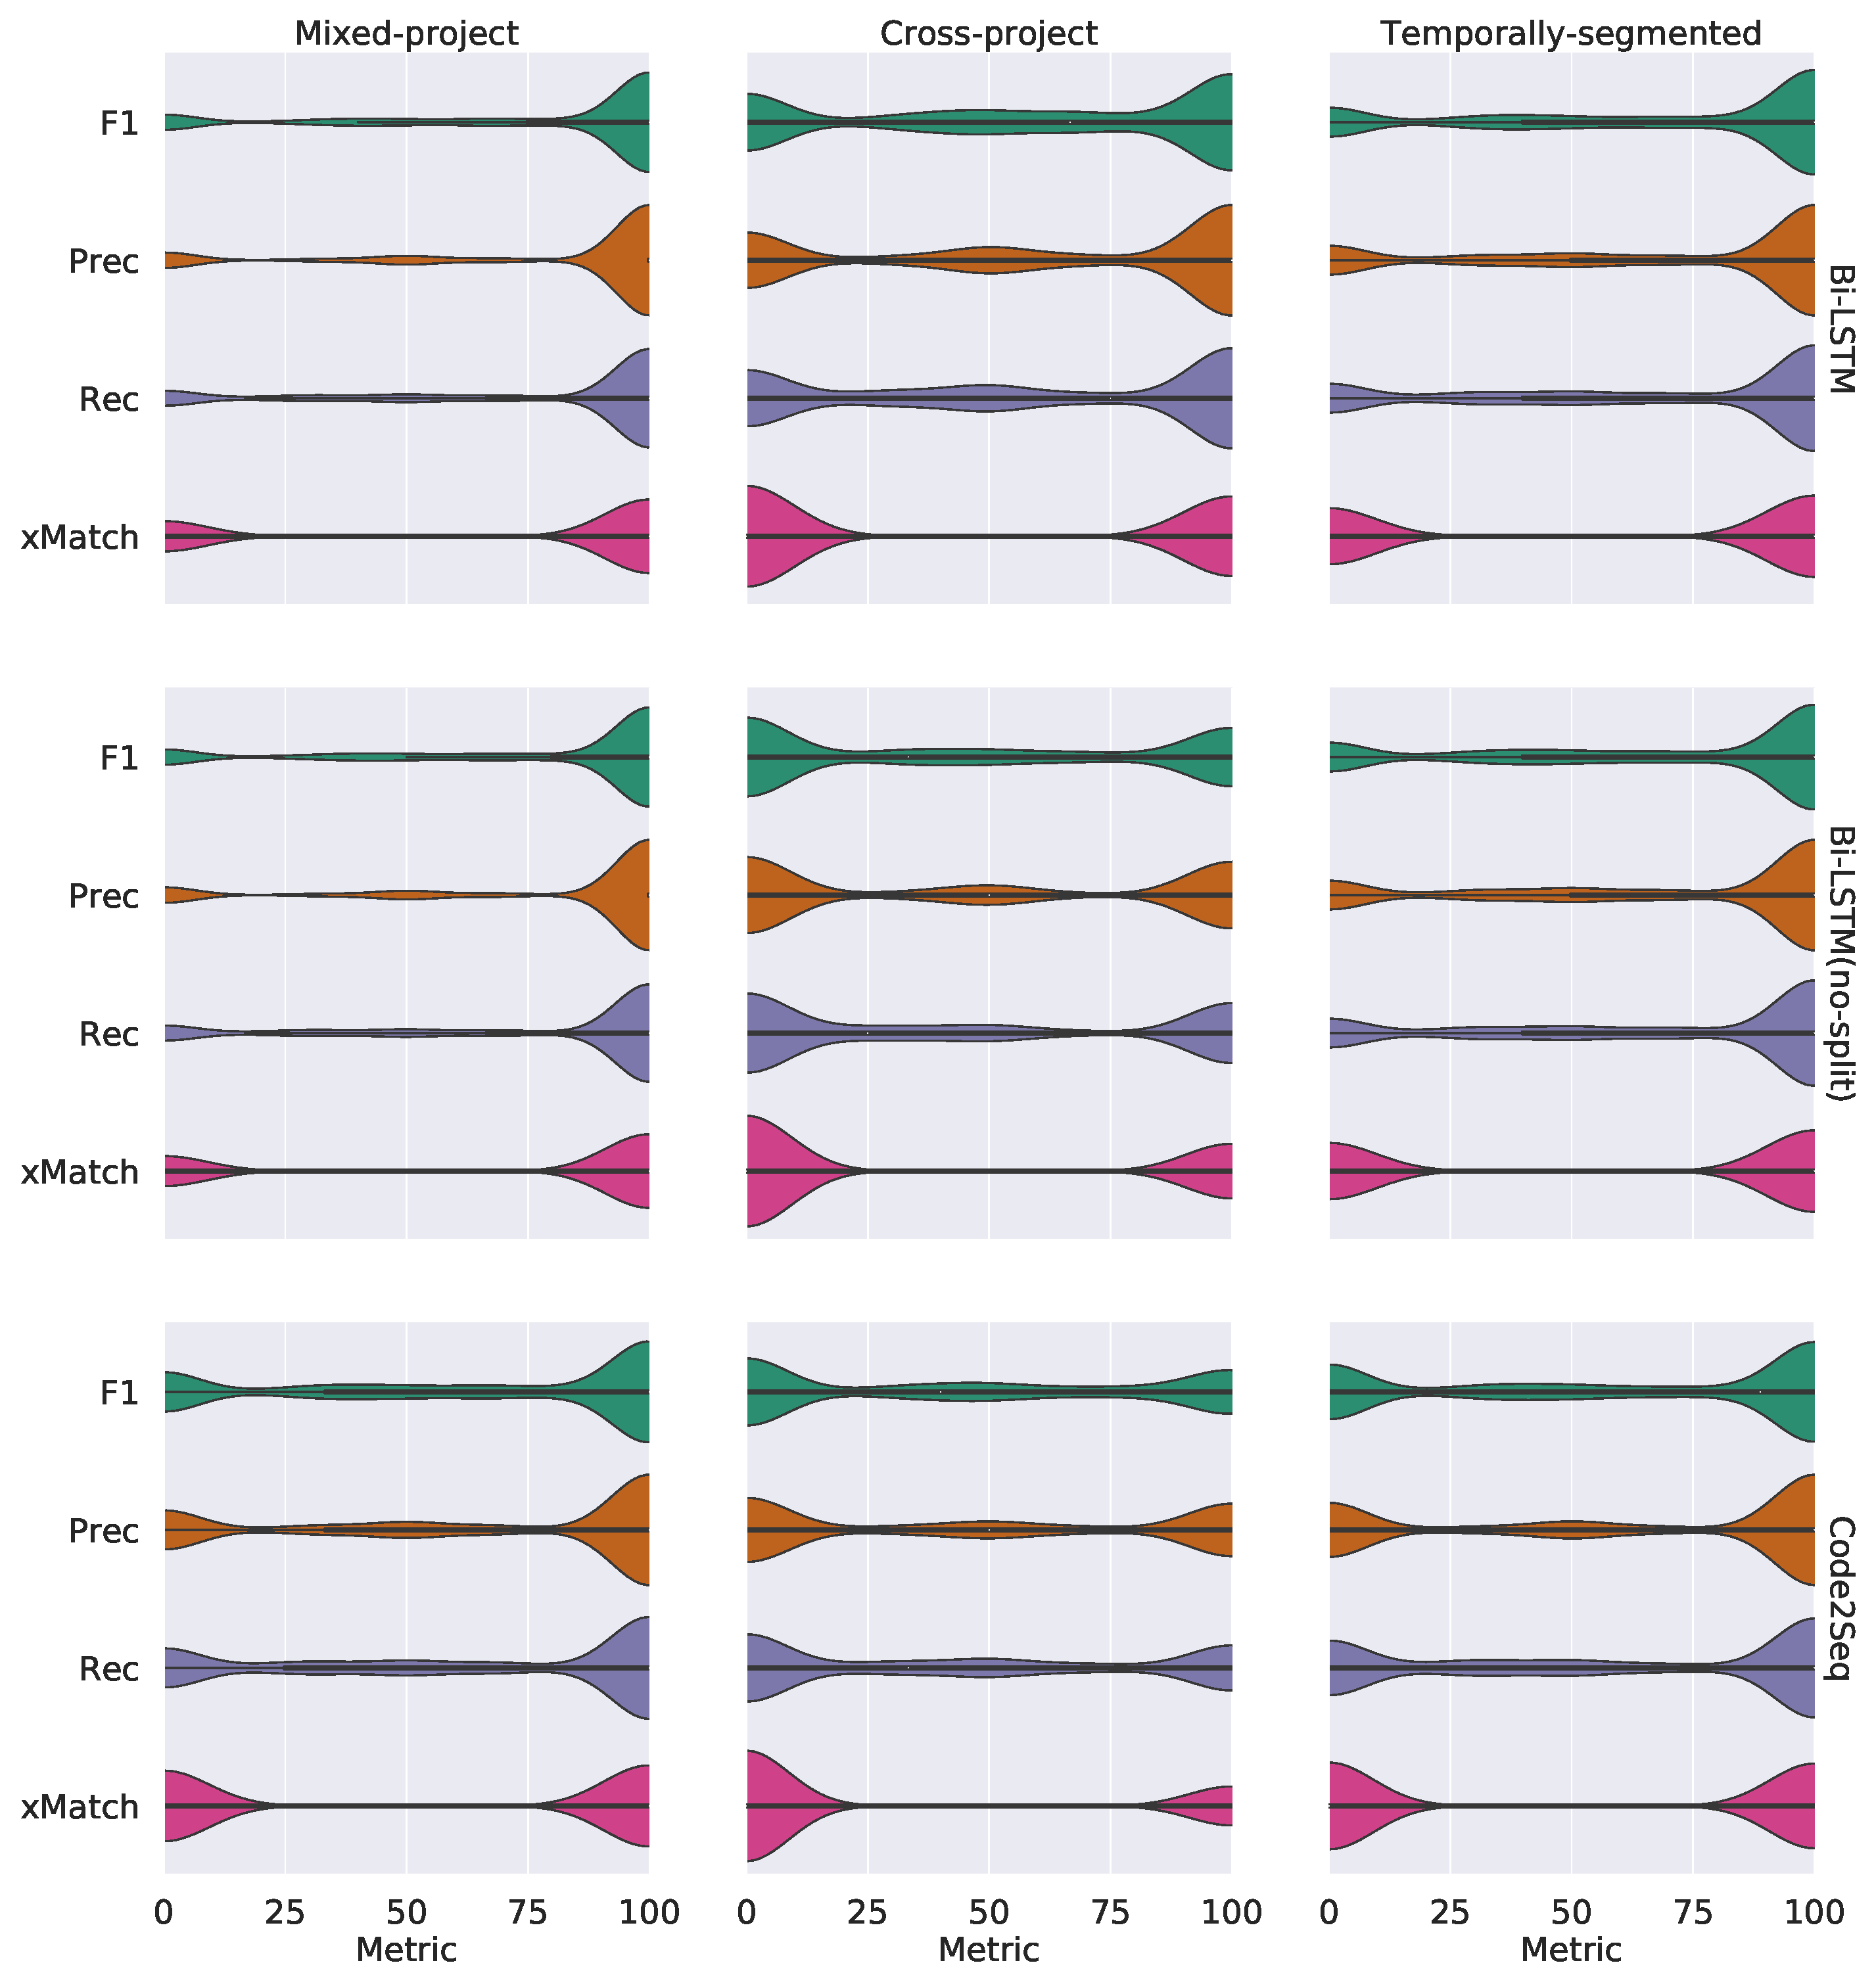
\includegraphics[width=\columnwidth]{figs/models-results-metrics-dist-MethNam.eps}
  \caption{Each violin plot shows the distribution of automated
    metrics on all examples in \test set.  Left to right: \mixedproj,
    \crossproj, and \evoaware \methodologies.  Top to bottom: the
    models for \methnam
    task. \label{fig:models-results-metrics-dist-MethNam}}
\end{figure}

\begin{figure}[t]
  \centering
  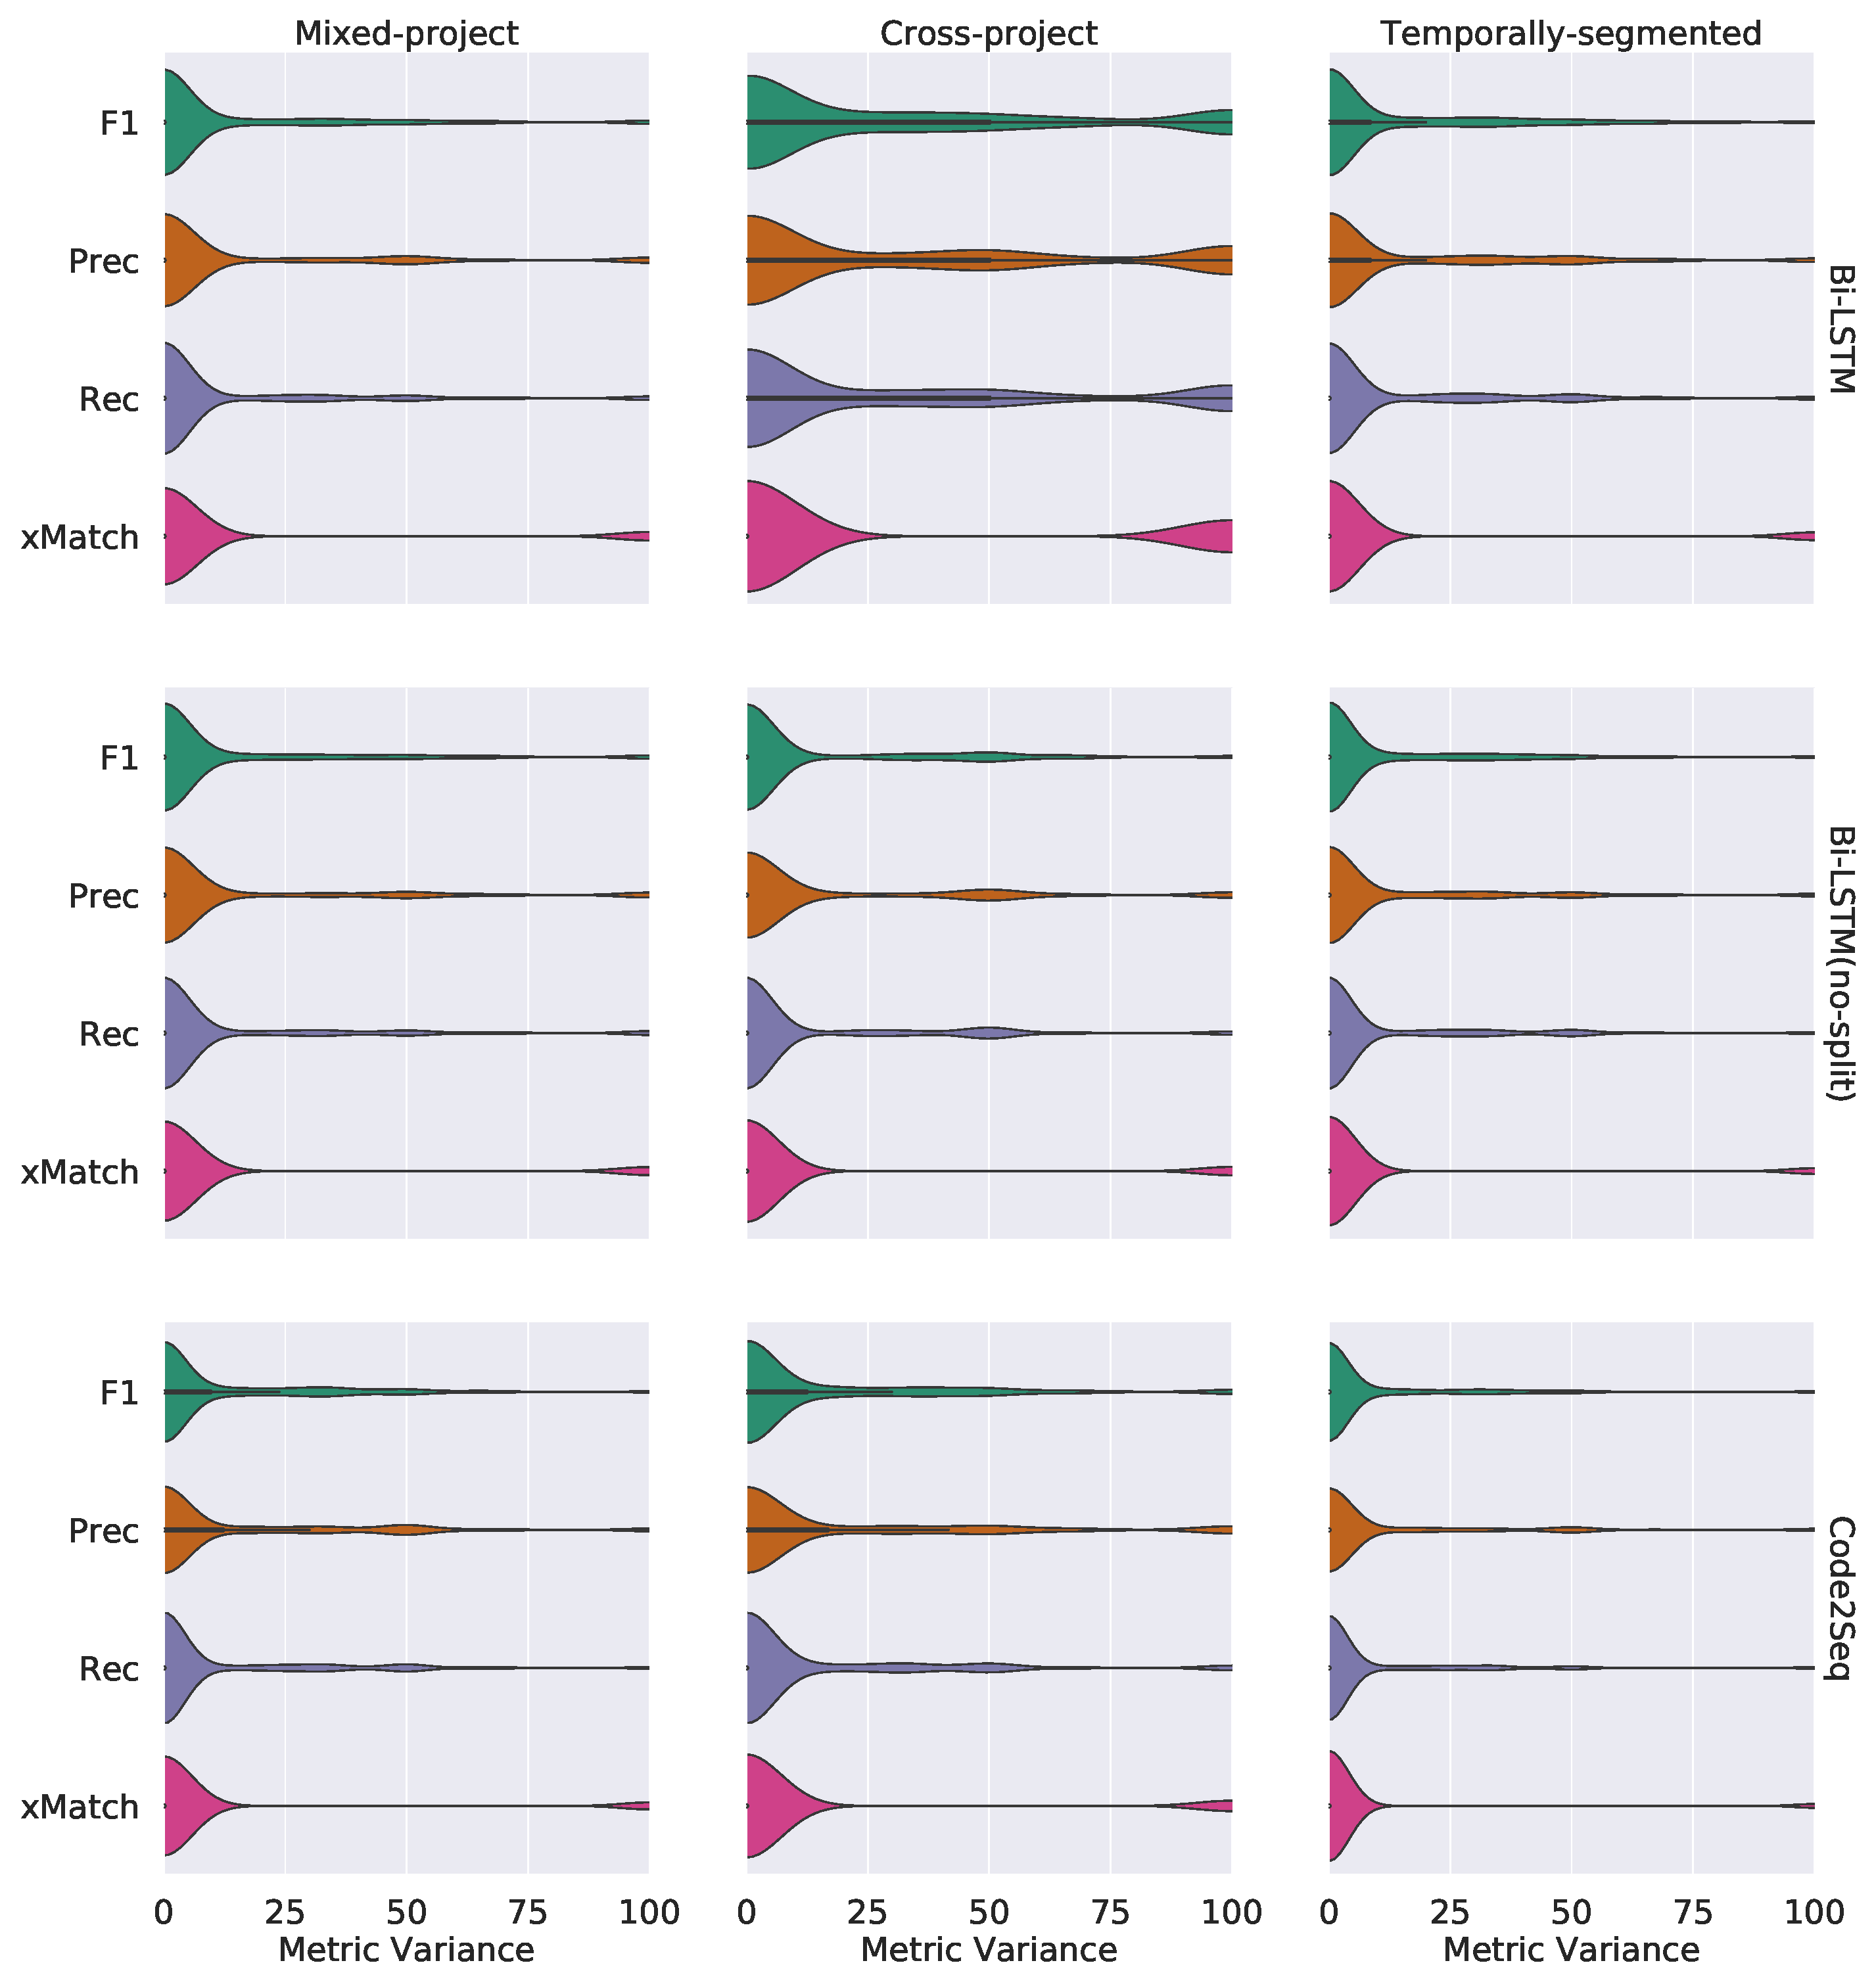
\includegraphics[width=\columnwidth]{figs/models-results-variance-dist-MethNam.eps}
  \caption{Each violin plot shows the distribution of the variances of
    automated metrics on all examples in \test set across \NumTrial
    trials.  Left to right: \mixedproj, \crossproj, and \evoaware
    \methodologies.  Top to bottom: the models for \methnam
    task. \label{fig:models-results-variance-dist-MethNam}}
\end{figure}

Figure~\ref{fig:models-results-metrics-dist-MethNam} shows the
distributions of automatic metrics on examples in \test set.
Figure~\ref{fig:models-results-variance-dist-MethNam} shows the
distributions of the variances of automated metrics on examples in
\test between \NumTrial different trials, where the variance is
calculated as the diff of the maximum value in \NumTrial trials and
minimum value in \NumTrial trials.


\subsection{Findings}
\label{sec:eval:findings}
From Table~\ref{}, models trained using \mixedproj \methodology and
\evoaware \methodology perform better in both automatic metrics than
\crossproj \methodology. This is because the using \mixedproj and
\evoaware \methodology models can learn from the
existing method and comment pairs within the projects so that the
model is able to generate comments that have similar styles or follow
the same rules. It has been shown by prior work that it is tough for
models to generalize between projects. All the models using \mixedproj
\methodology have better performance than \evoaware \methodology
probably because of the difference in the size of training data.
%Contradicted with Hu et al. ~\cite{}, \DeepCom does not outperform 
%\Seq2seq and \Seq2seqAtt uniformly in all the settings. DeepCom does
%worse than two baselines in mixed and cross proj setting but best in
%temporally setting.


% ========== The following tables are old before 20200827. They'll be either updated, replaced with plots, or removed

%
%% Automatically generated by pyutil.latex 

\begin{table*}
\begin{small}
\begin{center}
\caption{DeepCom results}
\begin{tabular}{l | c}
\toprule
  &BLEU-4 \\
\midrule
2013-2014-train
 & \UseMacro{deepcom-1314-bleu}
\\
2014-2015-train
 & \UseMacro{deepcom-1415-bleu}
\\
2015-2016-train
 & \UseMacro{deepcom-1516-bleu}
\\
2016-2017-train
 & \UseMacro{deepcom-1617-bleu}
\\
2017-2018-train
 & \UseMacro{deepcom-1718-bleu}
\\
\bottomrule
\end{tabular}
\end{center}
\end{small}
\vspace{\TVDatasetMetrics}
\end{table*}

%\begin{table*}
\begin{small}
\begin{center}
\caption{Results for Transformer}
\begin{tabular}{l | l}

\toprule

Training-Test & BLEU-4 \\

\midrule

Latest-Latest(epoch-20) &
\UseMacro{tr-lat-lat} \\
\midrule

Evolution-Latest(epoch-3) &
\UseMacro{tr-evo-lat} \\
\midrule

Evolution-Evolution(epoch-3) &
\UseMacro{tr-evo-evo} \\
\midrule

Latest-Evolution(epoch-18) &
\UseMacro{tr-lat-evo} \\
\midrule

\bottomrule

\end{tabular}
\end{center}
\end{small}
\vspace{\TVModels}
\end{table*}

%\begin{table*}
\begin{small}
\begin{center}
\caption{10 Projects}
\begin{tabular}{l}
\toprule
Projects \\
\midrule
   apache-commons-collections \\
google-guava\\
google-auto\\
rackerlabs-blueflood\\
jenkinsci-jenkins\\
dynjs-dynjs\\
spring-projects-spring-boot\\
oracle-graal\\
ReactiveX-RxJava\\
square-retrofit\\
\bottomrule
\end{tabular}
\end{center}
\end{small}
\vspace{\TVDatasetMetrics}
\end{table*}


%% 
%% Automatically generated by pyutil.latex 

\begin{table*}
\begin{small}
\begin{center}
\caption{Dataset statistics large (1000 projects)}
\begin{tabular}{l | r r r r r r r r}
\toprule
  &2013 & 2014 & 2015 & 2016 & 2017 & 2018 & 2019 & 2020 \\
\midrule
num-methods
 & \UseMacro{large-2013_Jan_1-num-methods}
 & \UseMacro{large-2014_Jan_1-num-methods}
 & \UseMacro{large-2015_Jan_1-num-methods}
 & \UseMacro{large-2016_Jan_1-num-methods}
 & \UseMacro{large-2017_Jan_1-num-methods}
 & \UseMacro{large-2018_Jan_1-num-methods}
 & \UseMacro{large-2019_Jan_1-num-methods}
 & \UseMacro{large-2020_Jan_1-num-methods}
\\
num-projs
 & \UseMacro{large-2013_Jan_1-num-projs}
 & \UseMacro{large-2014_Jan_1-num-projs}
 & \UseMacro{large-2015_Jan_1-num-projs}
 & \UseMacro{large-2016_Jan_1-num-projs}
 & \UseMacro{large-2017_Jan_1-num-projs}
 & \UseMacro{large-2018_Jan_1-num-projs}
 & \UseMacro{large-2019_Jan_1-num-projs}
 & \UseMacro{large-2020_Jan_1-num-projs}
\\
delta
 & \UseMacro{large-2013_Jan_1-delta}
 & \UseMacro{large-2014_Jan_1-delta}
 & \UseMacro{large-2015_Jan_1-delta}
 & \UseMacro{large-2016_Jan_1-delta}
 & \UseMacro{large-2017_Jan_1-delta}
 & \UseMacro{large-2018_Jan_1-delta}
 & \UseMacro{large-2019_Jan_1-delta}
 & \UseMacro{large-2020_Jan_1-delta}
\\
 after-filtered
 & N/A
 & \UseMacro{large-2013_Jan_1-2014_Jan_1-num-methods}
 & \UseMacro{large-2014_Jan_1-2015_Jan_1-num-methods}
 & \UseMacro{large-2015_Jan_1-2016_Jan_1-num-methods}
 & \UseMacro{large-2016_Jan_1-2017_Jan_1-num-methods}
 & \UseMacro{large-2017_Jan_1-2018_Jan_1-num-methods}
 & \UseMacro{large-2018_Jan_1-2019_Jan_1-num-methods}
 & \UseMacro{large-2019_Jan_1-2020_Jan_1-num-methods}
\\
\bottomrule
\end{tabular}
\end{center}
\end{small}
\vspace{\TVDatasetMetrics}
\end{table*}

%% 
%% Automatically generated by pyutil.latex 

\begin{table*}
\begin{small}
\begin{center}
\caption{Dataset statistics (10 projects)}
\begin{tabular}{l | r r r r r r r r}
\toprule
  &2013 & 2014 & 2015 & 2016 & 2017 & 2018 & 2019 & 2020 \\
\midrule
num-methods
 & \UseMacro{2013_Jan_1-num-methods}
 & \UseMacro{2014_Jan_1-num-methods}
 & \UseMacro{2015_Jan_1-num-methods}
 & \UseMacro{2016_Jan_1-num-methods}
 & \UseMacro{2017_Jan_1-num-methods}
 & \UseMacro{2018_Jan_1-num-methods}
 & \UseMacro{2019_Jan_1-num-methods}
 & \UseMacro{2020_Jan_1-num-methods}
\\
num-projs
 & \UseMacro{2013_Jan_1-num-projs}
 & \UseMacro{2014_Jan_1-num-projs}
 & \UseMacro{2015_Jan_1-num-projs}
 & \UseMacro{2016_Jan_1-num-projs}
 & \UseMacro{2017_Jan_1-num-projs}
 & \UseMacro{2018_Jan_1-num-projs}
 & \UseMacro{2019_Jan_1-num-projs}
 & \UseMacro{2020_Jan_1-num-projs}
\\
delta
 & \UseMacro{2013_Jan_1-delta}
 & \UseMacro{2014_Jan_1-delta}
 & \UseMacro{2015_Jan_1-delta}
 & \UseMacro{2016_Jan_1-delta}
 & \UseMacro{2017_Jan_1-delta}
 & \UseMacro{2018_Jan_1-delta}
 & \UseMacro{2019_Jan_1-delta}
 & \UseMacro{2020_Jan_1-delta}
\\
after-filtered
 & N/A
 & 4681
 & 3133
 & 5733
 & 6255
 & 9770
 & 6047
 & 6655
\\
\bottomrule
\end{tabular}
\end{center}
\end{small}
\vspace{\TVDatasetMetrics}
\end{table*}

%% 
%% Automatically generated by pyutil.latex 

\begin{table*}
\begin{small}
\begin{center}
\caption{method statistics after filtering (1000 projects)}
\begin{tabular}{l | c c c c c c c}
\toprule
 
 &
num-methods 
 &
len-avg 
 &
len-mode 
 &
len-median 
 &
len<100 
 &
len<150 
 &
len<200 
 \\
\midrule
2013-2014
 & \UseMacro{large-2013_Jan_1-2014_Jan_1-num-methods}
 & \UseMacro{large-2013_Jan_1-2014_Jan_1-method-tokens-avg}
 & \UseMacro{large-2013_Jan_1-2014_Jan_1-method-tokens-mode}
 & \UseMacro{large-2013_Jan_1-2014_Jan_1-method-tokens-median}
 & \UseMacro{large-2013_Jan_1-2014_Jan_1-method-tokens-less-100}
 & \UseMacro{large-2013_Jan_1-2014_Jan_1-method-tokens-less-150}
 & \UseMacro{large-2013_Jan_1-2014_Jan_1-method-tokens-less-200}
\\
2014-2015
 & \UseMacro{large-2014_Jan_1-2015_Jan_1-num-methods}
 & \UseMacro{large-2014_Jan_1-2015_Jan_1-method-tokens-avg}
 & \UseMacro{large-2014_Jan_1-2015_Jan_1-method-tokens-mode}
 & \UseMacro{large-2014_Jan_1-2015_Jan_1-method-tokens-median}
 & \UseMacro{large-2014_Jan_1-2015_Jan_1-method-tokens-less-100}
 & \UseMacro{large-2014_Jan_1-2015_Jan_1-method-tokens-less-150}
 & \UseMacro{large-2014_Jan_1-2015_Jan_1-method-tokens-less-200}
\\
2015-2016
 & \UseMacro{large-2015_Jan_1-2016_Jan_1-num-methods}
 & \UseMacro{large-2015_Jan_1-2016_Jan_1-method-tokens-avg}
 & \UseMacro{large-2015_Jan_1-2016_Jan_1-method-tokens-mode}
 & \UseMacro{large-2015_Jan_1-2016_Jan_1-method-tokens-median}
 & \UseMacro{large-2015_Jan_1-2016_Jan_1-method-tokens-less-100}
 & \UseMacro{large-2015_Jan_1-2016_Jan_1-method-tokens-less-150}
 & \UseMacro{large-2015_Jan_1-2016_Jan_1-method-tokens-less-200}
\\
2016-2017
 & \UseMacro{large-2016_Jan_1-2017_Jan_1-num-methods}
 & \UseMacro{large-2016_Jan_1-2017_Jan_1-method-tokens-avg}
 & \UseMacro{large-2016_Jan_1-2017_Jan_1-method-tokens-mode}
 & \UseMacro{large-2016_Jan_1-2017_Jan_1-method-tokens-median}
 & \UseMacro{large-2016_Jan_1-2017_Jan_1-method-tokens-less-100}
 & \UseMacro{large-2016_Jan_1-2017_Jan_1-method-tokens-less-150}
 & \UseMacro{large-2016_Jan_1-2017_Jan_1-method-tokens-less-200}
\\
2017-2018
 & \UseMacro{large-2017_Jan_1-2018_Jan_1-num-methods}
 & \UseMacro{large-2017_Jan_1-2018_Jan_1-method-tokens-avg}
 & \UseMacro{large-2017_Jan_1-2018_Jan_1-method-tokens-mode}
 & \UseMacro{large-2017_Jan_1-2018_Jan_1-method-tokens-median}
 & \UseMacro{large-2017_Jan_1-2018_Jan_1-method-tokens-less-100}
 & \UseMacro{large-2017_Jan_1-2018_Jan_1-method-tokens-less-150}
 & \UseMacro{large-2017_Jan_1-2018_Jan_1-method-tokens-less-200}
\\
2018-2019
 & \UseMacro{large-2018_Jan_1-2019_Jan_1-num-methods}
 & \UseMacro{large-2018_Jan_1-2019_Jan_1-method-tokens-avg}
 & \UseMacro{large-2018_Jan_1-2019_Jan_1-method-tokens-mode}
 & \UseMacro{large-2018_Jan_1-2019_Jan_1-method-tokens-median}
 & \UseMacro{large-2018_Jan_1-2019_Jan_1-method-tokens-less-100}
 & \UseMacro{large-2018_Jan_1-2019_Jan_1-method-tokens-less-150}
 & \UseMacro{large-2018_Jan_1-2019_Jan_1-method-tokens-less-200}
\\
2019-2020
 & \UseMacro{large-2019_Jan_1-2020_Jan_1-num-methods}
 & \UseMacro{large-2019_Jan_1-2020_Jan_1-method-tokens-avg}
 & \UseMacro{large-2019_Jan_1-2020_Jan_1-method-tokens-mode}
 & \UseMacro{large-2019_Jan_1-2020_Jan_1-method-tokens-median}
 & \UseMacro{large-2019_Jan_1-2020_Jan_1-method-tokens-less-100}
 & \UseMacro{large-2019_Jan_1-2020_Jan_1-method-tokens-less-150}
 & \UseMacro{large-2019_Jan_1-2020_Jan_1-method-tokens-less-200}
\\
\bottomrule
\end{tabular}
\end{center}
\end{small}
\vspace{\TVDatasetMetrics}
\end{table*}

%% 
%% Automatically generated by pyutil.latex 

\begin{table*}
\begin{small}
\begin{center}
\caption{method statistics after filtering (10 projects)}
\begin{tabular}{l | c c c c c c c}
\toprule
 
 &
num-methods 
 &
len-avg 
 &
len-mode 
 &
len-median 
 &
len<100 
 &
len<150 
 &
len<200 
 \\
\midrule
2013-2014
 & \UseMacro{2013_Jan_1-2014_Jan_1-num-methods}
 & \UseMacro{2013_Jan_1-2014_Jan_1-method-tokens-avg}
 & \UseMacro{2013_Jan_1-2014_Jan_1-method-tokens-mode}
 & \UseMacro{2013_Jan_1-2014_Jan_1-method-tokens-median}
 & \UseMacro{2013_Jan_1-2014_Jan_1-method-tokens-less-100}
 & \UseMacro{2013_Jan_1-2014_Jan_1-method-tokens-less-150}
 & \UseMacro{2013_Jan_1-2014_Jan_1-method-tokens-less-200}
\\
2014-2015
 & \UseMacro{2014_Jan_1-2015_Jan_1-num-methods}
 & \UseMacro{2014_Jan_1-2015_Jan_1-method-tokens-avg}
 & \UseMacro{2014_Jan_1-2015_Jan_1-method-tokens-mode}
 & \UseMacro{2014_Jan_1-2015_Jan_1-method-tokens-median}
 & \UseMacro{2014_Jan_1-2015_Jan_1-method-tokens-less-100}
 & \UseMacro{2014_Jan_1-2015_Jan_1-method-tokens-less-150}
 & \UseMacro{2014_Jan_1-2015_Jan_1-method-tokens-less-200}
\\
2015-2016
 & \UseMacro{2015_Jan_1-2016_Jan_1-num-methods}
 & \UseMacro{2015_Jan_1-2016_Jan_1-method-tokens-avg}
 & \UseMacro{2015_Jan_1-2016_Jan_1-method-tokens-mode}
 & \UseMacro{2015_Jan_1-2016_Jan_1-method-tokens-median}
 & \UseMacro{2015_Jan_1-2016_Jan_1-method-tokens-less-100}
 & \UseMacro{2015_Jan_1-2016_Jan_1-method-tokens-less-150}
 & \UseMacro{2015_Jan_1-2016_Jan_1-method-tokens-less-200}
\\
2016-2017
 & \UseMacro{2016_Jan_1-2017_Jan_1-num-methods}
 & \UseMacro{2016_Jan_1-2017_Jan_1-method-tokens-avg}
 & \UseMacro{2016_Jan_1-2017_Jan_1-method-tokens-mode}
 & \UseMacro{2016_Jan_1-2017_Jan_1-method-tokens-median}
 & \UseMacro{2016_Jan_1-2017_Jan_1-method-tokens-less-100}
 & \UseMacro{2016_Jan_1-2017_Jan_1-method-tokens-less-150}
 & \UseMacro{2016_Jan_1-2017_Jan_1-method-tokens-less-200}
\\
2017-2018
 & \UseMacro{2017_Jan_1-2018_Jan_1-num-methods}
 & \UseMacro{2017_Jan_1-2018_Jan_1-method-tokens-avg}
 & \UseMacro{2017_Jan_1-2018_Jan_1-method-tokens-mode}
 & \UseMacro{2017_Jan_1-2018_Jan_1-method-tokens-median}
 & \UseMacro{2017_Jan_1-2018_Jan_1-method-tokens-less-100}
 & \UseMacro{2017_Jan_1-2018_Jan_1-method-tokens-less-150}
 & \UseMacro{2017_Jan_1-2018_Jan_1-method-tokens-less-200}
\\
2018-2019
 & \UseMacro{2018_Jan_1-2019_Jan_1-num-methods}
 & \UseMacro{2018_Jan_1-2019_Jan_1-method-tokens-avg}
 & \UseMacro{2018_Jan_1-2019_Jan_1-method-tokens-mode}
 & \UseMacro{2018_Jan_1-2019_Jan_1-method-tokens-median}
 & \UseMacro{2018_Jan_1-2019_Jan_1-method-tokens-less-100}
 & \UseMacro{2018_Jan_1-2019_Jan_1-method-tokens-less-150}
 & \UseMacro{2018_Jan_1-2019_Jan_1-method-tokens-less-200}
\\
2019-2020
 & \UseMacro{2019_Jan_1-2020_Jan_1-num-methods}
 & \UseMacro{2019_Jan_1-2020_Jan_1-method-tokens-avg}
 & \UseMacro{2019_Jan_1-2020_Jan_1-method-tokens-mode}
 & \UseMacro{2019_Jan_1-2020_Jan_1-method-tokens-median}
 & \UseMacro{2019_Jan_1-2020_Jan_1-method-tokens-less-100}
 & \UseMacro{2019_Jan_1-2020_Jan_1-method-tokens-less-150}
 & \UseMacro{2019_Jan_1-2020_Jan_1-method-tokens-less-200}
\\
\bottomrule
\end{tabular}
\end{center}
\end{small}
\vspace{\TVDatasetMetrics}
\end{table*}

%% 
%% Automatically generated by pyutil.latex 

\begin{table*}
\begin{small}
\begin{center}
\caption{comment statistics after filtering (1000 projects)}
\begin{tabular}{l | c c c c c c c}
\toprule
 
 &
num-methods 
 &
len-avg 
 &
len-mode 
 &
len-median 
 &
len<20 
 &
len<30 
 &
len<50 
 \\
\midrule
2013-2014
 & \UseMacro{large-2013_Jan_1-2014_Jan_1-num-methods}
 & \UseMacro{large-2013_Jan_1-2014_Jan_1-comment-tokens-avg}
 & \UseMacro{large-2013_Jan_1-2014_Jan_1-comment-tokens-mode}
 & \UseMacro{large-2013_Jan_1-2014_Jan_1-comment-tokens-median}
 & \UseMacro{large-2013_Jan_1-2014_Jan_1-comment-tokens-less-20}
 & \UseMacro{large-2013_Jan_1-2014_Jan_1-comment-tokens-less-30}
 & \UseMacro{large-2013_Jan_1-2014_Jan_1-comment-tokens-less-50}
\\
2014-2015
 & \UseMacro{large-2014_Jan_1-2015_Jan_1-num-methods}
 & \UseMacro{large-2014_Jan_1-2015_Jan_1-comment-tokens-avg}
 & \UseMacro{large-2014_Jan_1-2015_Jan_1-comment-tokens-mode}
 & \UseMacro{large-2014_Jan_1-2015_Jan_1-comment-tokens-median}
 & \UseMacro{large-2014_Jan_1-2015_Jan_1-comment-tokens-less-20}
 & \UseMacro{large-2014_Jan_1-2015_Jan_1-comment-tokens-less-30}
 & \UseMacro{large-2014_Jan_1-2015_Jan_1-comment-tokens-less-50}
\\
2015-2016
 & \UseMacro{large-2015_Jan_1-2016_Jan_1-num-methods}
 & \UseMacro{large-2015_Jan_1-2016_Jan_1-comment-tokens-avg}
 & \UseMacro{large-2015_Jan_1-2016_Jan_1-comment-tokens-mode}
 & \UseMacro{large-2015_Jan_1-2016_Jan_1-comment-tokens-median}
 & \UseMacro{large-2015_Jan_1-2016_Jan_1-comment-tokens-less-20}
 & \UseMacro{large-2015_Jan_1-2016_Jan_1-comment-tokens-less-30}
 & \UseMacro{large-2015_Jan_1-2016_Jan_1-comment-tokens-less-50}
\\
2016-2017
 & \UseMacro{large-2016_Jan_1-2017_Jan_1-num-methods}
 & \UseMacro{large-2016_Jan_1-2017_Jan_1-comment-tokens-avg}
 & \UseMacro{large-2016_Jan_1-2017_Jan_1-comment-tokens-mode}
 & \UseMacro{large-2016_Jan_1-2017_Jan_1-comment-tokens-median}
 & \UseMacro{large-2016_Jan_1-2017_Jan_1-comment-tokens-less-20}
 & \UseMacro{large-2016_Jan_1-2017_Jan_1-comment-tokens-less-30}
 & \UseMacro{large-2016_Jan_1-2017_Jan_1-comment-tokens-less-50}
\\
2017-2018
 & \UseMacro{large-2017_Jan_1-2018_Jan_1-num-methods}
 & \UseMacro{large-2017_Jan_1-2018_Jan_1-comment-tokens-avg}
 & \UseMacro{large-2017_Jan_1-2018_Jan_1-comment-tokens-mode}
 & \UseMacro{large-2017_Jan_1-2018_Jan_1-comment-tokens-median}
 & \UseMacro{large-2017_Jan_1-2018_Jan_1-comment-tokens-less-20}
 & \UseMacro{large-2017_Jan_1-2018_Jan_1-comment-tokens-less-30}
 & \UseMacro{large-2017_Jan_1-2018_Jan_1-comment-tokens-less-50}
\\
2018-2019
 & \UseMacro{large-2018_Jan_1-2019_Jan_1-num-methods}
 & \UseMacro{large-2018_Jan_1-2019_Jan_1-comment-tokens-avg}
 & \UseMacro{large-2018_Jan_1-2019_Jan_1-comment-tokens-mode}
 & \UseMacro{large-2018_Jan_1-2019_Jan_1-comment-tokens-median}
 & \UseMacro{large-2018_Jan_1-2019_Jan_1-comment-tokens-less-20}
 & \UseMacro{large-2018_Jan_1-2019_Jan_1-comment-tokens-less-30}
 & \UseMacro{large-2018_Jan_1-2019_Jan_1-comment-tokens-less-50}
\\
2019-2020
 & \UseMacro{large-2019_Jan_1-2020_Jan_1-num-methods}
 & \UseMacro{large-2019_Jan_1-2020_Jan_1-comment-tokens-avg}
 & \UseMacro{large-2019_Jan_1-2020_Jan_1-comment-tokens-mode}
 & \UseMacro{large-2019_Jan_1-2020_Jan_1-comment-tokens-median}
 & \UseMacro{large-2019_Jan_1-2020_Jan_1-comment-tokens-less-20}
 & \UseMacro{large-2019_Jan_1-2020_Jan_1-comment-tokens-less-30}
 & \UseMacro{large-2019_Jan_1-2020_Jan_1-comment-tokens-less-50}
\\
\bottomrule
\end{tabular}
\end{center}
\end{small}
\vspace{\TVDatasetMetrics}
\end{table*}

%% 
%% Automatically generated by pyutil.latex 

\begin{table*}
\begin{small}
\begin{center}
\caption{comment statistics after filtering (10 projects)}
\begin{tabular}{l | c c c c c c c}
\toprule
 
 &
num-methods 
 &
len-avg 
 &
len-mode 
 &
len-median 
 &
len<20 
 &
len<30 
 &
len<50 
 \\
\midrule
2013-2014
 & \UseMacro{2013_Jan_1-2014_Jan_1-num-methods}
 & \UseMacro{2013_Jan_1-2014_Jan_1-comment-tokens-avg}
 & \UseMacro{2013_Jan_1-2014_Jan_1-comment-tokens-mode}
 & \UseMacro{2013_Jan_1-2014_Jan_1-comment-tokens-median}
 & \UseMacro{2013_Jan_1-2014_Jan_1-comment-tokens-less-20}
 & \UseMacro{2013_Jan_1-2014_Jan_1-comment-tokens-less-30}
 & \UseMacro{2013_Jan_1-2014_Jan_1-comment-tokens-less-50}
\\
2014-2015
 & \UseMacro{2014_Jan_1-2015_Jan_1-num-methods}
 & \UseMacro{2014_Jan_1-2015_Jan_1-comment-tokens-avg}
 & \UseMacro{2014_Jan_1-2015_Jan_1-comment-tokens-mode}
 & \UseMacro{2014_Jan_1-2015_Jan_1-comment-tokens-median}
 & \UseMacro{2014_Jan_1-2015_Jan_1-comment-tokens-less-20}
 & \UseMacro{2014_Jan_1-2015_Jan_1-comment-tokens-less-30}
 & \UseMacro{2014_Jan_1-2015_Jan_1-comment-tokens-less-50}
\\
2015-2016
 & \UseMacro{2015_Jan_1-2016_Jan_1-num-methods}
 & \UseMacro{2015_Jan_1-2016_Jan_1-comment-tokens-avg}
 & \UseMacro{2015_Jan_1-2016_Jan_1-comment-tokens-mode}
 & \UseMacro{2015_Jan_1-2016_Jan_1-comment-tokens-median}
 & \UseMacro{2015_Jan_1-2016_Jan_1-comment-tokens-less-20}
 & \UseMacro{2015_Jan_1-2016_Jan_1-comment-tokens-less-30}
 & \UseMacro{2015_Jan_1-2016_Jan_1-comment-tokens-less-50}
\\
2016-2017
 & \UseMacro{2016_Jan_1-2017_Jan_1-num-methods}
 & \UseMacro{2016_Jan_1-2017_Jan_1-comment-tokens-avg}
 & \UseMacro{2016_Jan_1-2017_Jan_1-comment-tokens-mode}
 & \UseMacro{2016_Jan_1-2017_Jan_1-comment-tokens-median}
 & \UseMacro{2016_Jan_1-2017_Jan_1-comment-tokens-less-20}
 & \UseMacro{2016_Jan_1-2017_Jan_1-comment-tokens-less-30}
 & \UseMacro{2016_Jan_1-2017_Jan_1-comment-tokens-less-50}
\\
2017-2018
 & \UseMacro{2017_Jan_1-2018_Jan_1-num-methods}
 & \UseMacro{2017_Jan_1-2018_Jan_1-comment-tokens-avg}
 & \UseMacro{2017_Jan_1-2018_Jan_1-comment-tokens-mode}
 & \UseMacro{2017_Jan_1-2018_Jan_1-comment-tokens-median}
 & \UseMacro{2017_Jan_1-2018_Jan_1-comment-tokens-less-20}
 & \UseMacro{2017_Jan_1-2018_Jan_1-comment-tokens-less-30}
 & \UseMacro{2017_Jan_1-2018_Jan_1-comment-tokens-less-50}
\\
2018-2019
 & \UseMacro{2018_Jan_1-2019_Jan_1-num-methods}
 & \UseMacro{2018_Jan_1-2019_Jan_1-comment-tokens-avg}
 & \UseMacro{2018_Jan_1-2019_Jan_1-comment-tokens-mode}
 & \UseMacro{2018_Jan_1-2019_Jan_1-comment-tokens-median}
 & \UseMacro{2018_Jan_1-2019_Jan_1-comment-tokens-less-20}
 & \UseMacro{2018_Jan_1-2019_Jan_1-comment-tokens-less-30}
 & \UseMacro{2018_Jan_1-2019_Jan_1-comment-tokens-less-50}
\\
2019-2020
 & \UseMacro{2019_Jan_1-2020_Jan_1-num-methods}
 & \UseMacro{2019_Jan_1-2020_Jan_1-comment-tokens-avg}
 & \UseMacro{2019_Jan_1-2020_Jan_1-comment-tokens-mode}
 & \UseMacro{2019_Jan_1-2020_Jan_1-comment-tokens-median}
 & \UseMacro{2019_Jan_1-2020_Jan_1-comment-tokens-less-20}
 & \UseMacro{2019_Jan_1-2020_Jan_1-comment-tokens-less-30}
 & \UseMacro{2019_Jan_1-2020_Jan_1-comment-tokens-less-50}
\\
\bottomrule
\end{tabular}
\end{center}
\end{small}
\vspace{\TVDatasetMetrics}
\end{table*}

%% 
%% Automatically generated by pyutil.latex 

\begin{table*}
\begin{small}
\begin{center}
\caption{DeepCom results}
\begin{tabular}{l | c}
\toprule
  &BLEU-4 \\
\midrule
2013-2014-train
 & \UseMacro{deepcom-1314-bleu}
\\
2014-2015-train
 & \UseMacro{deepcom-1415-bleu}
\\
2015-2016-train
 & \UseMacro{deepcom-1516-bleu}
\\
2016-2017-train
 & \UseMacro{deepcom-1617-bleu}
\\
2017-2018-train
 & \UseMacro{deepcom-1718-bleu}
\\
\bottomrule
\end{tabular}
\end{center}
\end{small}
\vspace{\TVDatasetMetrics}
\end{table*}

%% 
%% Automatically generated by pyutil.latex 

\begin{table*}
\begin{small}
\begin{center}
\caption{DeepCom results}
\begin{tabular}{l | c | c |c |c |c}
\toprule
 Time-BLEU-4
& Seq2seq
& Seq2seqAtt
& DeepCom-SBT
& DeepCom-Preorder
& DeepCom
\\
\midrule
2013-2014-train
 & \UseMacro{seq2seq-1314-bleu}
 & \UseMacro{seq2seqatt-1314-bleu}
 & \UseMacro{deepcom-sbt-1314-bleu}
 & \UseMacro{deepcom-preorder-1314-bleu}
 & \UseMacro{deepcom-1314-bleu}
\\
2014-2015-train
 & \UseMacro{seq2seq-1415-bleu}
 & \UseMacro{seq2seqatt-1415-bleu}
 & \UseMacro{deepcom-sbt-1415-bleu}
 & \UseMacro{deepcom-preorder-1415-bleu}
 & \UseMacro{deepcom-1415-bleu}
\\
2015-2016-train
 & \UseMacro{seq2seq-1516-bleu}
 & \UseMacro{seq2seqatt-1516-bleu}
 & \UseMacro{deepcom-sbt-1516-bleu}
 & \UseMacro{deepcom-preorder-1516-bleu}
 & \UseMacro{deepcom-1516-bleu}
\\
2016-2017-train
 & \UseMacro{seq2seq-1617-bleu}
 & \UseMacro{seq2seqatt-1617-bleu}
 & \UseMacro{deepcom-sbt-1617-bleu}
 & \UseMacro{deepcom-preorder-1617-bleu}
 & \UseMacro{deepcom-1617-bleu}
\\
2017-2018-train
 & \UseMacro{seq2seq-1718-bleu}
 & \UseMacro{seq2seqatt-1718-bleu}
 & \UseMacro{deepcom-sbt-1718-bleu}
 & \UseMacro{deepcom-preorder-1718-bleu}
 & \UseMacro{deepcom-1718-bleu}
\\
\bottomrule
\end{tabular}
\end{center}
\end{small}
\vspace{\TVDatasetMetrics}
\end{table*}

%% 
%% Automatically generated by pyutil.latex

\begin{table*}
\begin{small}
\begin{center}
\caption{DeepCom results on latest data}
\begin{tabular}{l | c | c |c |c |c}
\toprule
 Time-BLEU-4
& Seq2seq
& Seq2seqAtt
& DeepCom-SBT
& DeepCom-Preorder
& DeepCom
\\
\midrule
2020-train
 & 23.67
 & 24.17
 & 11.71
 & 8.15
 & 25.27
\\
\bottomrule
\end{tabular}
\end{center}
\end{small}
\vspace{\TVDatasetMetrics}
\end{table*}
%% 
%% Automatically generated by pyutil.latex 

\begin{table*}
\begin{small}
\begin{center}
\caption{Method naming statistics after filtering}
\begin{tabular}{l | c | c}
\toprule
 
 &
num-methods
&
code-len-avg
 \\
\midrule
2013-2014
 & \UseMacro{debug-beta-2013_Jan_1-2014_Jan_1-num-methods}
 & \UseMacro{debug-beta-2013-avg-len}
\\
2014-2015
 & \UseMacro{debug-beta-2014_Jan_1-2015_Jan_1-num-methods}
& \UseMacro{debug-beta-2014-avg-len}
\\
2015-2016
 & \UseMacro{debug-beta-2015_Jan_1-2016_Jan_1-num-methods}
& \UseMacro{debug-beta-2015-avg-len}
\\
2016-2017
 & \UseMacro{debug-beta-2016_Jan_1-2017_Jan_1-num-methods}
& \UseMacro{debug-beta-2016-avg-len}
\\
2017-2018
 & \UseMacro{debug-beta-2017_Jan_1-2018_Jan_1-num-methods}
& \UseMacro{debug-beta-2017-avg-len}
\\
2018-2019
 & \UseMacro{debug-beta-2018_Jan_1-2019_Jan_1-num-methods}
& \UseMacro{debug-beta-2018-avg-len}
\\
2019-2020
 & \UseMacro{debug-beta-2019_Jan_1-2020_Jan_1-num-methods}
 & \UseMacro{debug-beta-2019-avg-len}
\\
\bottomrule
\end{tabular}
\end{center}
\end{small}
\vspace{\TVDatasetMetrics}
\end{table*}

%% %% Automatically generated by pyutil.latex

\begin{table*}
\begin{small}
\begin{center}
\caption{Method naming task results}
\begin{tabular}{l | c | c}
\toprule
 Time-F1
 & Code2Seq
 & BiLSTM
\\
\midrule
2013-2014-train
 & \UseMacro{code2seq-debug-1314-F1}
 & 0.57
\\
2014-2015-train
 & \UseMacro{code2seq-debug-1415-F1}
 & 0.55
\\
2015-2016-train
 & \UseMacro{code2seq-debug-1516-F1}
 & 0.65
\\
2016-2017-train
 & \UseMacro{code2seq-debug-1617-F1}
 & 0.63
\\
2017-2018-train
 & \UseMacro{code2seq-debug-1718-F1}
 & 0.65
\\
latest-train
 & \UseMacro{code2seq-debug-latest-F1}
 & 0.58
\\
\bottomrule
\end{tabular}
\end{center}
\end{small}
\vspace{\TVDatasetMetrics}
\end{table*}

%% 
%% Automatically generated by pyutil.latex 

\begin{table*}
\begin{small}
\begin{center}
\caption{Comment-generation results}
\begin{tabular}{l|c|c|c|c}
\toprule
 Time-Bleu-4
& Seq2seq
& Seq2seqAtt
& DeepCom-SBT
& DeepCom
\\
\midrule
2013-2014-train
 & \UseMacro{seq2seq-1314-train-bleu}
 & \UseMacro{seq2seqatt-1314-train-bleu}
 & \UseMacro{deepcom-sbt-1314-train-bleu}
 & \UseMacro{deepcom-1314-train-bleu}
\\
2014-2015-train
 & \UseMacro{seq2seq-1415-train-bleu}
 & \UseMacro{seq2seqatt-1415-train-bleu}
 & \UseMacro{deepcom-sbt-1415-train-bleu}
 & \UseMacro{deepcom-1415-train-bleu}
\\
2015-2016-train
 & \UseMacro{seq2seq-1516-train-bleu}
 & \UseMacro{seq2seqatt-1516-train-bleu}
 & \UseMacro{deepcom-sbt-1516-train-bleu}
 & \UseMacro{deepcom-1516-train-bleu}
\\
2016-2017-train
 & \UseMacro{seq2seq-1617-train-bleu}
 & \UseMacro{seq2seqatt-1617-train-bleu}
 & \UseMacro{deepcom-sbt-1617-train-bleu}
 & \UseMacro{deepcom-1617-train-bleu}
\\
2017-2018-train
 & \UseMacro{seq2seq-1718-train-bleu}
 & \UseMacro{seq2seqatt-1718-train-bleu}
 & \UseMacro{deepcom-sbt-1718-train-bleu}
 & \UseMacro{deepcom-1718-train-bleu}
\\
2020-train
 & \UseMacro{seq2seq-latest-bleu}
 & \UseMacro{seq2seqatt-latest-bleu}
 & \UseMacro{deepcom-sbt-latest-bleu}
 & \UseMacro{deepcom-latest-bleu}
\\
\bottomrule
\end{tabular}
\end{center}
\end{small}
\vspace{\TVDatasetMetrics}
\end{table*}

%% 
%% Automatically generated by pyutil.latex 

\begin{table*}
\begin{small}
\begin{center}
\caption{Method-naming results}
\begin{tabular}{l|c|c|c|c|c|c|c|c|c}
\toprule
 \multirow{2}{*}{Time-Metrics}
& \multicolumn{3}{c}{Bi-LSTM}
& \multicolumn{3}{c}{no-split-Bi-LSTM}
& \multicolumn{3}{c}{Code2Seq}
\\
& precision
& recall
& f1
& precision
& recall
& f1
& precision
& recall
& f1
\\
\midrule
2013-2014-train
 & \UseMacro{bi-lstm-1314-train-precision}
 & \UseMacro{bi-lstm-1314-train-recall}
 & \UseMacro{bi-lstm-1314-train-f1}
 & \UseMacro{no-split-bi-lstm-1314-train-precision}
 & \UseMacro{no-split-bi-lstm-1314-train-recall}
 & \UseMacro{no-split-bi-lstm-1314-train-f1}
 & \UseMacro{code2seq-1314-train-precision}
 & \UseMacro{code2seq-1314-train-recall}
 & \UseMacro{code2seq-1314-train-f1}
\\
2014-2015-train
 & \UseMacro{bi-lstm-1415-train-precision}
 & \UseMacro{bi-lstm-1415-train-recall}
 & \UseMacro{bi-lstm-1415-train-f1}
 & \UseMacro{no-split-bi-lstm-1415-train-precision}
 & \UseMacro{no-split-bi-lstm-1415-train-recall}
 & \UseMacro{no-split-bi-lstm-1415-train-f1}
 & \UseMacro{code2seq-1415-train-precision}
 & \UseMacro{code2seq-1415-train-recall}
 & \UseMacro{code2seq-1415-train-f1}
\\
2015-2016-train
 & \UseMacro{bi-lstm-1516-train-precision}
 & \UseMacro{bi-lstm-1516-train-recall}
 & \UseMacro{bi-lstm-1516-train-f1}
 & \UseMacro{no-split-bi-lstm-1516-train-precision}
 & \UseMacro{no-split-bi-lstm-1516-train-recall}
 & \UseMacro{no-split-bi-lstm-1516-train-f1}
 & \UseMacro{code2seq-1516-train-precision}
 & \UseMacro{code2seq-1516-train-recall}
 & \UseMacro{code2seq-1516-train-f1}
\\
2016-2017-train
 & \UseMacro{bi-lstm-1617-train-precision}
 & \UseMacro{bi-lstm-1617-train-recall}
 & \UseMacro{bi-lstm-1617-train-f1}
 & \UseMacro{no-split-bi-lstm-1617-train-precision}
 & \UseMacro{no-split-bi-lstm-1617-train-recall}
 & \UseMacro{no-split-bi-lstm-1617-train-f1}
 & \UseMacro{code2seq-1617-train-precision}
 & \UseMacro{code2seq-1617-train-recall}
 & \UseMacro{code2seq-1617-train-f1}
\\
2017-2018-train
 & \UseMacro{bi-lstm-1718-train-precision}
 & \UseMacro{bi-lstm-1718-train-recall}
 & \UseMacro{bi-lstm-1718-train-f1}
 & \UseMacro{no-split-bi-lstm-1718-train-precision}
 & \UseMacro{no-split-bi-lstm-1718-train-recall}
 & \UseMacro{no-split-bi-lstm-1718-train-f1}
 & \UseMacro{code2seq-1718-train-precision}
 & \UseMacro{code2seq-1718-train-recall}
 & \UseMacro{code2seq-1718-train-f1}
\\
latest-mixed
 & \UseMacro{bi-lstm-latest-precision}
 & \UseMacro{bi-lstm-latest-recall}
 & \UseMacro{bi-lstm-latest-f1}
 & \UseMacro{no-split-bi-lstm-latest-precision}
 & \UseMacro{no-split-bi-lstm-latest-recall}
 & \UseMacro{no-split-bi-lstm-latest-f1}
 & \UseMacro{code2seq-latest-precision}
 & \UseMacro{code2seq-latest-recall}
 & \UseMacro{code2seq-latest-f1}
\\
latest-cross-project
 & \UseMacro{bi-lstm-cross-proj-latest-precision}
 & \UseMacro{bi-lstm-cross-proj-latest-recall}
 & \UseMacro{bi-lstm-cross-proj-latest-f1}
 & \UseMacro{no-split-bi-lstm-cross-proj-latest-precision}
 & \UseMacro{no-split-bi-lstm-cross-proj-latest-recall}
 & \UseMacro{no-split-bi-lstm-cross-proj-latest-f1}
 & \UseMacro{code2seq-cross-proj-latest-precision}
 & \UseMacro{code2seq-cross-proj-latest-recall}
 & \UseMacro{code2seq-cross-proj-latest-f1}
\\
\bottomrule
\end{tabular}
\end{center}
\end{small}
\vspace{\TVDatasetMetrics}
\end{table*}

